\documentclass[letterpaper,12pt]{article} %Modifica el tipo de documento y el tamaño de la letra.
\usepackage[utf8]{inputenc} %Formato UTF-8 para caracteres especiales.
\usepackage[shortlabels]{enumitem}
\usepackage[spanish,mexico]{babel} 
\usepackage{amsmath,amssymb,amsfonts,latexsym,cancel}
\usepackage{hyperref}
\usepackage{wrapfig}
\usepackage[rflt]{floatflt}
\usepackage[pdftex]{graphicx}
\usepackage{fancyhdr} %Paquete para el header y el formato de la portada. No sugiero borrarlo!
\usepackage{float}
\usepackage{longtable,multirow,booktabs}
\usepackage{cite}
\usepackage{verbatim}
\usepackage{multicol}
\usepackage{caption}
\usepackage{subcaption}
\usepackage[]{sidecap}
\usepackage{adjustbox}
\usepackage{parskip}
\usepackage{enumitem}
\usepackage{tikz}
\usepackage{lipsum}
\usepackage[]{xcolor}
\usepackage{soul}
\usepackage{minted}

% FORMATO DE LA PÁGINA
\textheight = 21cm %Medidas de la  página
\textwidth = 18cm  %Medidas de la página
\topmargin = -2cm  %Medidas de la página    
\oddsidemargin = -0.8cm %Medidas de la página
\pagestyle{fancy} %Diseño de la página
\setlength{\parindent}{12pt}

% FORMATO DE LA PORTADA
\fancyhf{}
\lhead{Facultad de Ingeniería}%%LeftHead
\chead{
\includegraphics[width=1cm, height=1cm]{figurasPortada/escudofi_rojo.jpg}}%%CenterHead
%\lfoot{USM}
\rhead{PROTECO}%%RightHead

\setlength{\columnsep}{4mm}%Comandos para el formato de la página.
%\setlength{\parindent}{4em}%Sangría al comenzar un nuevo párrafo.
\setlength{\parindent}{0.5in}
%\setlength{\parindent}{4em}%Sangría al comenzar un nuevo párrafo.
%\setlength{\parskip}{1em}%Distancia entre párrafos.
\renewcommand{\baselinestretch}{1.2}% Espacio entre línea y línea o interlineado.
\setlength{\headheight}{33pt}
\fancyfoot[C,CO]{\thepage}


\begin{document}

\thispagestyle{empty}
\begin{figure}[ht]
\minipage{0.87\textwidth}
    
\includegraphics[width=2cm]{figurasPortada/escudofi_rojo.jpg}
\endminipage
\minipage{0.32\textwidth}
    
\includegraphics[height = 2.25cm ,width=2cm]{figurasPortada/escudounam_azul.jpg}
\endminipage
    %%\vspace{-1cm}
\end{figure}

\vspace{0.07cm}

\begin{center}
{\scshape\LARGE \textbf{Universidad Nacional Autónoma de México} \par}
{\scshape\Large Facultad de Ingeniería\par}

{\Large Programa de Tecnología en Cómputo}

 {\Large Curso: Linux}

\vspace{0.5cm}

% Restauramos el interlineado:
\begin{center}
    {\LARGE  \bfseries{Proyecto Final} \\}
{\LARGE\bfseries Documentación ProtoShell\par}
\vspace{0.5cm}
    \LARGE	{ \textbf{Impartió:}}\\%% \textbf son negritas
\large		{Brian Jassiel Bautista Pérez}

\large {Abraham Galindo Ruiz}

\large {Juan Ángeles Hernández}

\vspace{0.5cm}

\LARGE	{ \textbf{Alumnos:}}\\%% \textbf son negritas

\normalsize		{Carrasco Meza Alan Michel}

\normalsize	 {García Acevedo Jonathan Enrique}

\vspace{0.5cm}

{\large \textit{Generación 44 - Semestre: 2023-2}}

{\Large Fecha de entrega: 22 de abril del 2023\par}
\end{center}

\end{center}
\newpage
\tableofcontents
\newpage

\section{Introducción}
Shell script es un lenguaje de programación ampliamente utilizado en diversos campo de la computación. Es particularmente útil para hacer uso de los sistemas operativos UNIX-like (Linux o macOS), al igual que mantener servidores con dichos sistemas operativos.

ProtoShell es un proyecto en el que se hace uso de Shell script para realizar tareas como : \textbf{*LISTA DE COSAS QUE PUDIMOS ACABAR DE LA SHELL*}. Esto con la finalidad de profundizar los conocimientos adquiridos a lo largo del curso de Linux y aplicar lo aprendido.

En este archivo se explica el funcionamiento y utilización de cada script que compone a la ProtoShell con la finalidad de que se evidencie el trabajo realizado por lo prebecarios y se oriente a los usuarios sobre el correcto uso de este software.

\section{Desarrollo}

\subsection{ProtoBash.sh}

ProtoBash es el documento 'base', en el cual se pueden observar cada una de las funcionalidades del proyecto, como lo son el prompt en el que se va a mostrar el usuario y en que carpeta o directorio en el que se encuentra el usuario, siendo una instrucción que requiere en todo momento nuestro shell script.

Además de cumplir con una sentencia '\textbf{case}' con varias opciones, las cuales son las diferentes funcionalidades que en el presente documento se van a ir explicando.

\begin{figure}[H]
    \centering
    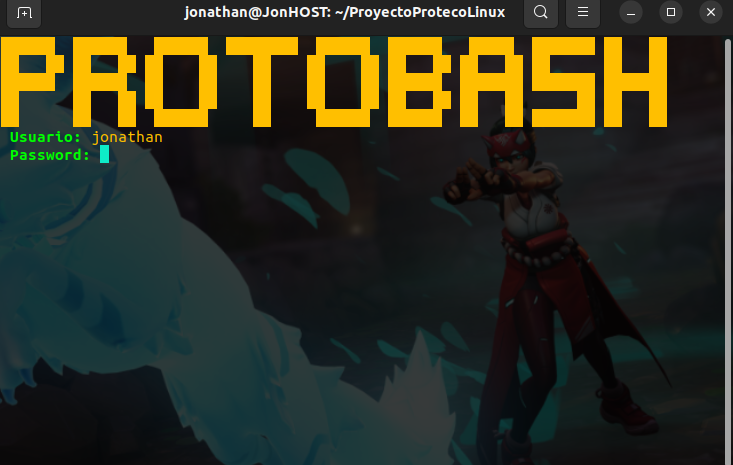
\includegraphics[width=0.5\textwidth]{figurasShell/ProtoBash1.png}
\end{figure}

%%%%%%%%%%%%%%%%%%%%%
% Para poner imágenes es con los siguientes comandos:
% \begin{figure}
%    \centering
%    \includegraphics[width=0.5\textwidth]{ <dirección de imagen, overleaf te lo debe sugerir> }
% \end{figure}
%%%%%%%%%%%%%%%%%%%%%

\subsection{Infosis.sh}

En el archivo Infosis.sh podemos encontrar lo siguiente sobre el sistema

La información sobre la memoria RAM.

\begin{minted}{bash}
$free -t --mega; grep 'MemTotal' /proc/meminfo; grep 'SwapTotal' /proc/meminfo $
\end{minted}

La arquitectura con la cual esta constituida la computadora en cuestión

\begin{minted}{bash}
$uname -m; $
\end{minted}
    Por último, la identificación de versión del sistema operativo:

\begin{minted}{bash}
$lsb_release -idc $
\end{minted}

\begin{figure}[H]
    \centering
    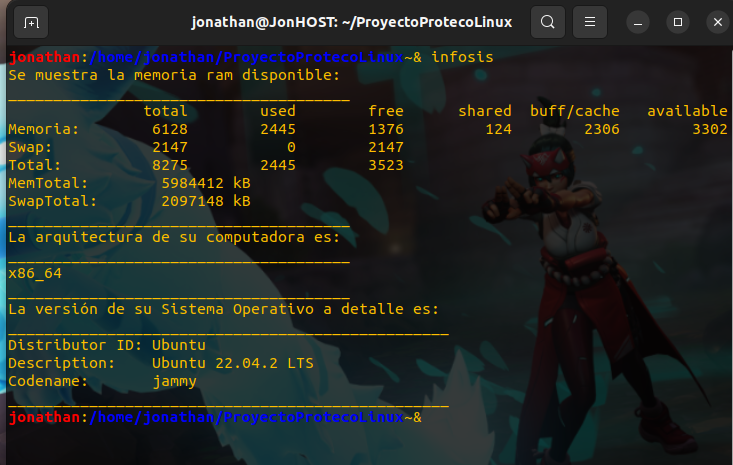
\includegraphics[width=0.5\textwidth]{figurasShell/InfoSis.png}
\end{figure}

\subsection{busqueda.sh}
La presente sección nos ayuda a lograr una búsqueda a partir de los parámetros ingresados por el usuario los cuales son:

El archivo a buscar por nombre con extensión de este:

\begin{minted}{bash}
printf "Archivo a buscar: "

read archivoBuscado
\end{minted}
\begin{figure}[H]
    \centering
    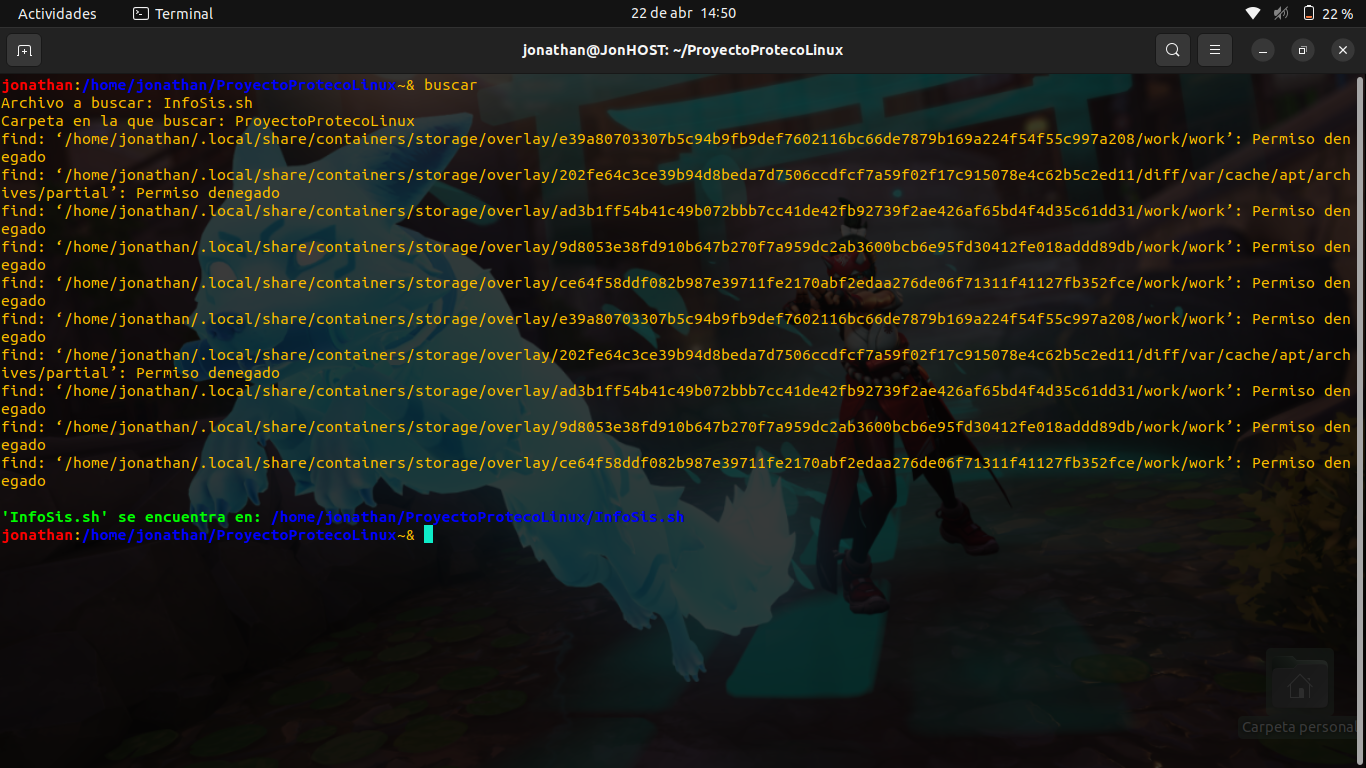
\includegraphics[width=0.5\textwidth]{figurasShell/Buscar1.png}
\end{figure}
El directorio donde se va a buscar, Aquí es suficiente con que se precise el nombre de la carpeta. Ingresar rutas relativas o absulutas producirá un error en la búsqueda.
    
\begin{minted}{bash}
printf "Carpeta en la que buscar: "

read carpetaBusqueda
\end{minted}

Una vez teniendo estos parámetros ingresados por el usuario, lo consiguiente se puede iniciar por la función buscarArchivo los cuales usan estos parámetros.

Se usa dentro de la función buscar archivo, transformándola en una variable, el comando find para el que usan como parámetros el primer punto donde se va a hacer la búsqueda
\begin{minted}{bash}
        "/home/$USER"
\end{minted}

con la bandera la cual nos afirma que la búsqueda va a hacer mediante el nombre 

\begin{minted}{bash}
-name
\end{minted}

y concluir con la variable que anteriormente se inicializo y se le dio el valor por parte del usuario para lograr la búsqueda mediante ese nombre.

\begin{minted}{bash}
"$carpetaBusqueda"
\end{minted}

Logrando así un código final como es el siguiente de este comando:

\begin{minted}{bash}
find "/home/$USER" -name "$carpetaBusqueda"
\end{minted}

Una vez teniendo estos valores definidos podemos empezar a realizar la búsqueda, aunque de inicio lo que se evalúa es si es que lo que se busca existe.

\begin{minted}{bash}
        if [[ -d "$direccionDirectorio" ]]; then
\end{minted}

ara continuar entonces con la búsqueda, teniendo que cuenta que se va a dar un nuevo valor para poder lograr y determinar si en verdad se logró la búsqueda

\begin{minted}{bash}
direccionArchivo=$(find "/home/$USER" -name "$archivoBuscado")

if [[ -f "$direccionArchivo" ]]
then
    printf "\n$G\'$archivoBuscado\' se encuentra en: $B$direccionArchivo\n"
else
    printf "\n$G\'$archivoBuscado\' $R no se encuentra$W en la carpeta $B$carpetaBusqueda\n"
fi
    
else
    printf "\nLa carpeta $B$carpetaBusqueda$R no se ha encontrado\n"
fi
\end{minted}

\begin{figure}[H]
    \centering
    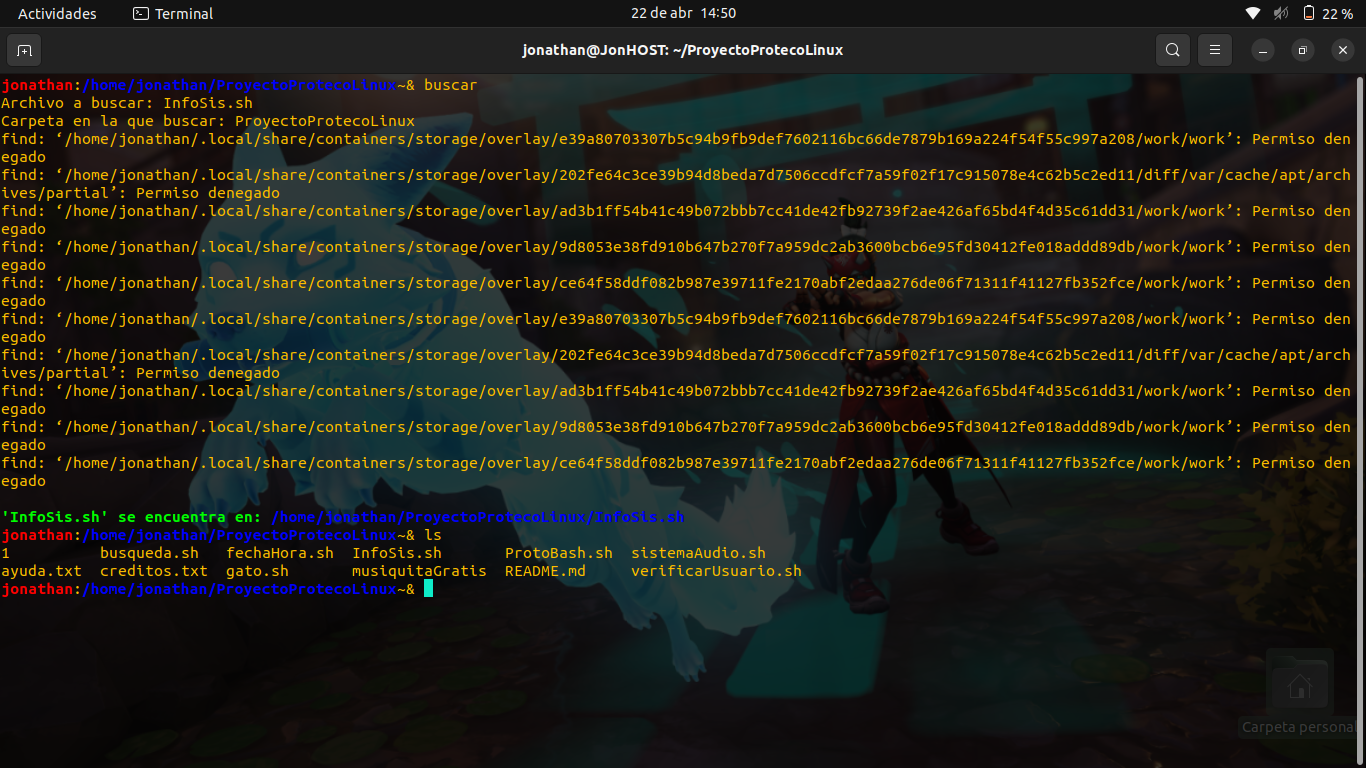
\includegraphics[width=0.5\textwidth]{figurasShell/Buscar2.png}
\end{figure}

\subsection{fechaHora.sh}

En la presente sección podemos observar dos cosas, la indicación de los colores que se van a dar para la impresión de la fecha:

\begin{minted}{bash}
    # Colores
    R='\033[1;31m'
    G='\033[1;32m'
    B='\033[1;34m'
    W='\033[0m'
\end{minted}

y la segunda parte que nos muestra en formatos definidos y con ayuda de las variables designadas para el color, la fecha en tipo dd/mm/aa con la hora en formato HH:MM:SS

\begin{minted}{bash}
    printf "$R Fecha:\t$W%(%d/%m/%Y)T\n"
    printf "$R Hora:\t$W%(%H:%M:%S2)T\n"
\end{minted}

\begin{figure}[H]
    \centering
    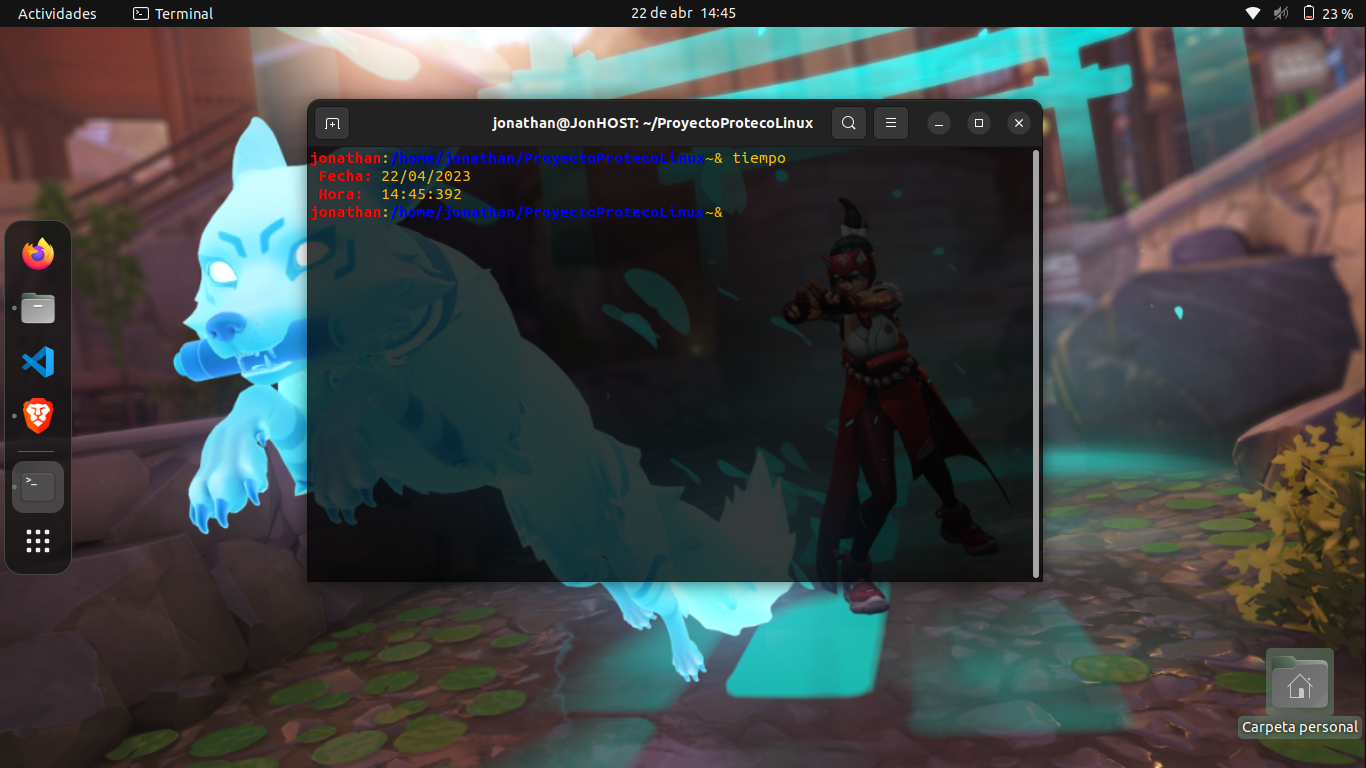
\includegraphics[width=0.5\textwidth]{figurasShell/Tiempo.png}
\end{figure}

\subsection{gato.sh}

    Se declara en un arreglo los valores que simbolizan cada casilla

\begin{minted}{bash}
    s=([1]=1 [2]=2 [3]=3 [4]=4 [5]=5 [6]=6 [7]=7 [8]=8 [9]=9)
\end{minted}
\begin{figure}[H]
    \centering
    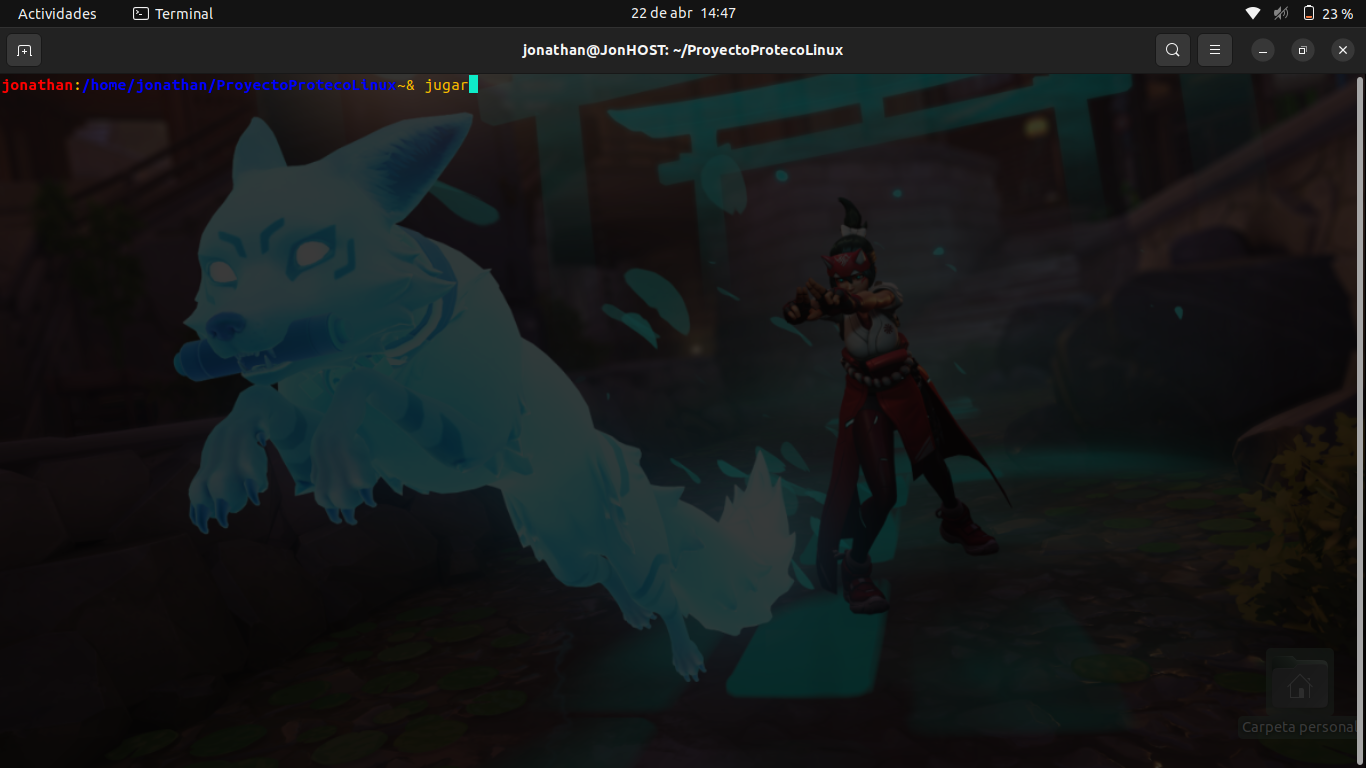
\includegraphics[width=0.5\textwidth]{figurasShell/Jugar1.png}
\end{figure}

    Símbolos para cada jugador
\begin{minted}{bash}
    SIMBOLO_JUGADOR1=X
    SIMBOLO_JUGADOR2=O
\end{minted}
    Función para dibujar el tablero

\begin{minted}{bash}
    dibujarTablero() {
	   echo "Jugador 1: ${SIMBOLO_JUGADOR1}, Jugador 2: ${SIMBOLO_JUGADOR2}"
	   echo " ${s[7]} | ${s[8]} | ${s[9]} "
	   echo "---+---+---"
	   echo " ${s[4]} | ${s[5]} | ${s[6]} "
	   echo "---+---+---"
	   echo " ${s[1]} | ${s[2]} | ${s[3]} "
    }
\end{minted}

\begin{figure}[H]
    \centering
    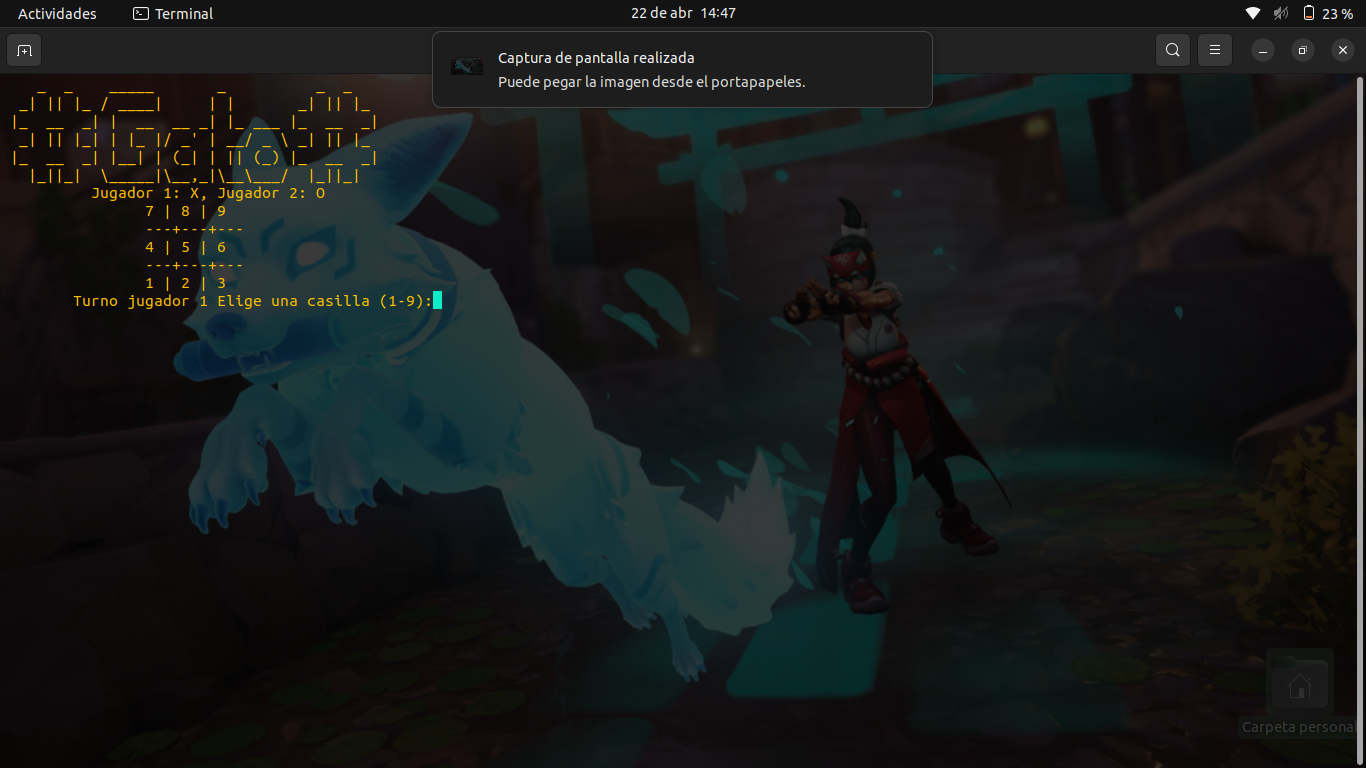
\includegraphics[width=0.5\textwidth]{figurasShell/Jugar2.png}
\end{figure}

    Expresión regular para verificar que el valor este entre 1 y 9
\begin{minted}{bash}
    RANGO_NUM='^[1-9]$'
\end{minted}
    Función para pedirle al jugador 1 su entrada

    \begin{figure}[H]
        \centering
        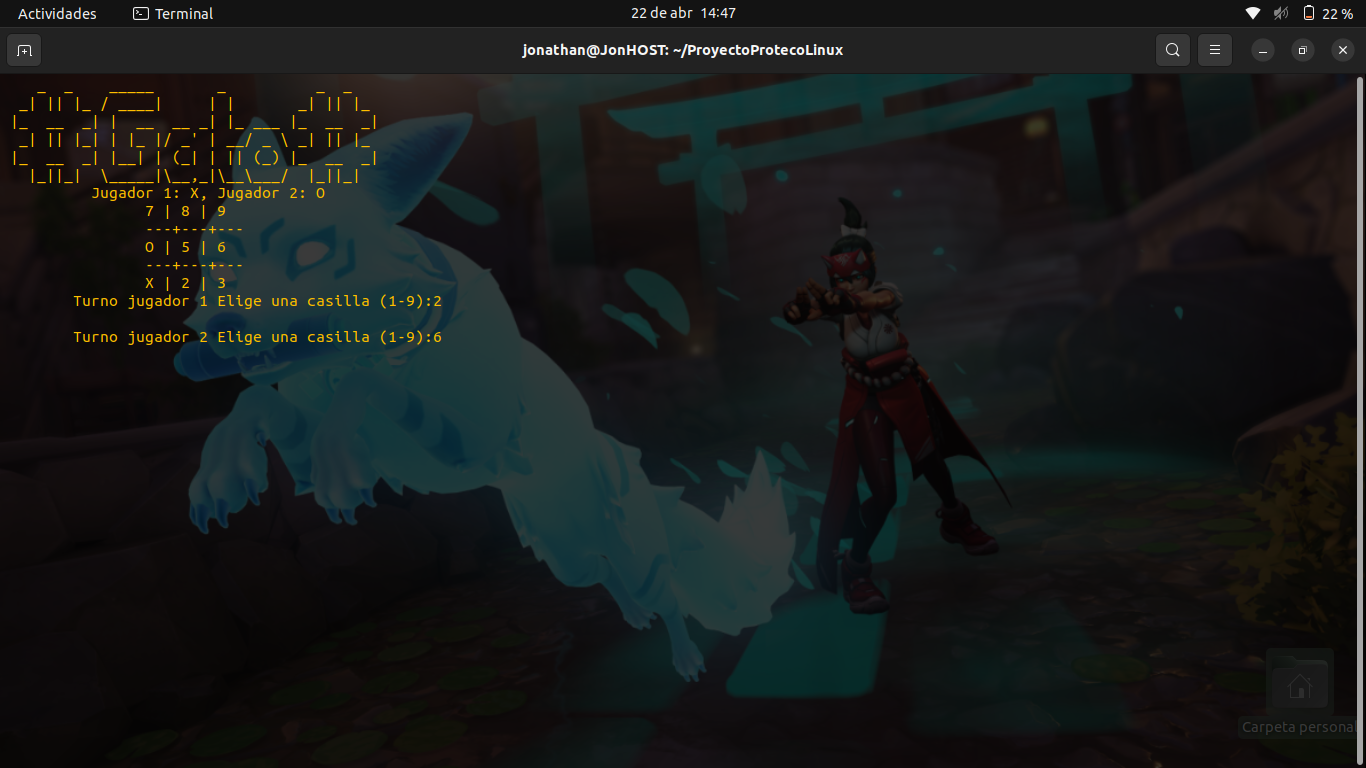
\includegraphics[width=0.5\textwidth]{figurasShell/Jugar3.png}
    \end{figure}
\begin{minted}{bash}
    Turno_jugador1() {
        printf "Enter your choice (1-9):"
        read casilla
        if ! [[ $casilla =~ $RANGO_NUM ]]; then
            echo "Debes escoger un numero entre 1 y 9"
                Turno_jugador1
        fi
        if ! [[ ${s[$casilla]} =~ $RANGO_NUM ]]; then
            echo "Casilla ocupada"
                Turno_jugador1
        fi
        s[$casilla]=$SIMBOLO_JUGADOR1
    }
\end{minted}
    Función para pedirle al jugador 2 su entrada

    \begin{figure}[H]
        \centering
        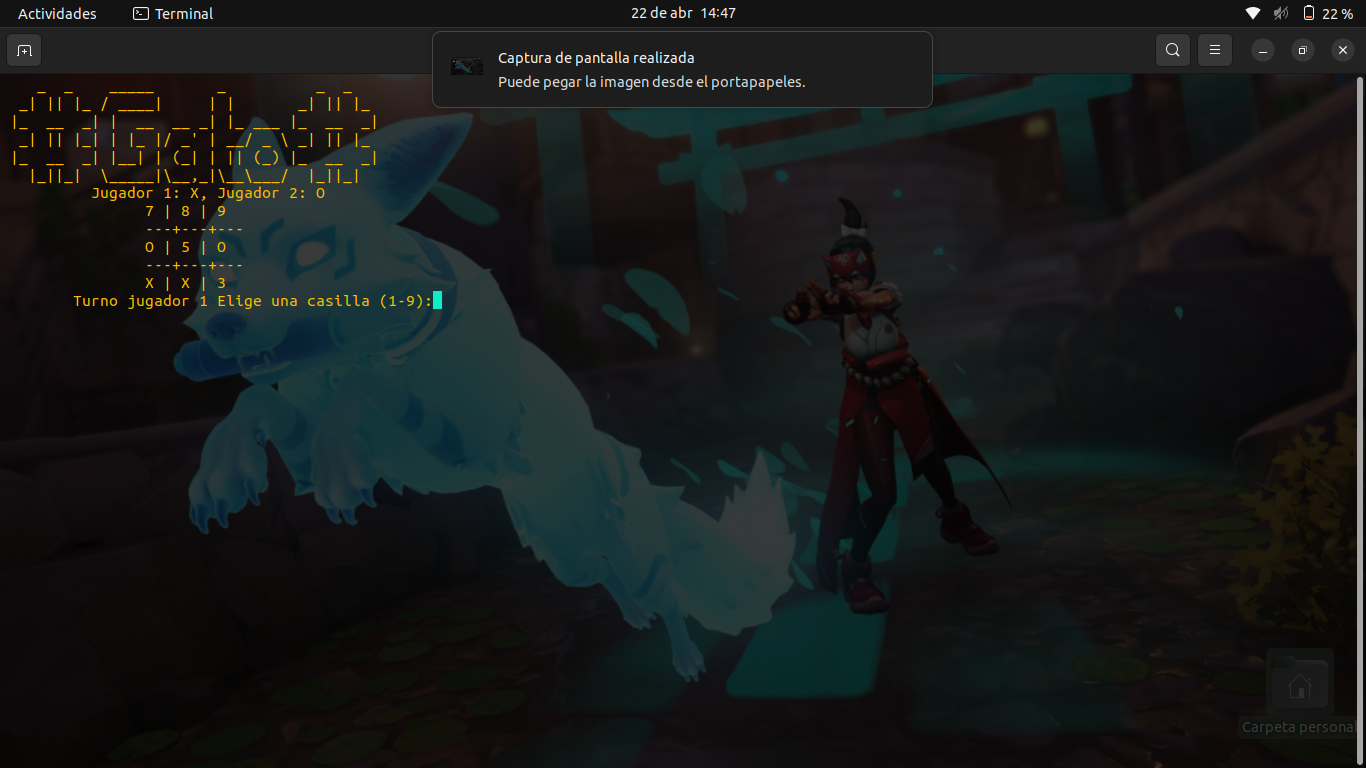
\includegraphics[width=0.5\textwidth]{figurasShell/Jugar4.png}
    \end{figure}
    
\begin{minted}{bash}
    Turno_jugador2(){
        printf "Enter your choice (1-9):"
        read casilla
        if ! [[ $casilla =~ $RANGO_NUM ]]; then
            echo "Debes escoger un numero 1 y 9"
		Turno_jugador2
	fi
	if ! [[ ${s[$casilla]} =~ $RANGO_NUM ]]; then
            echo "Casilla ocupada"
		Turno_jugador2
	fi
	s[$casilla]=$SIMBOLO_JUGADOR2
    }
\end{minted}
    Función para saber qué jugador se debe imprimir

    \begin{figure}[H]
        \centering
        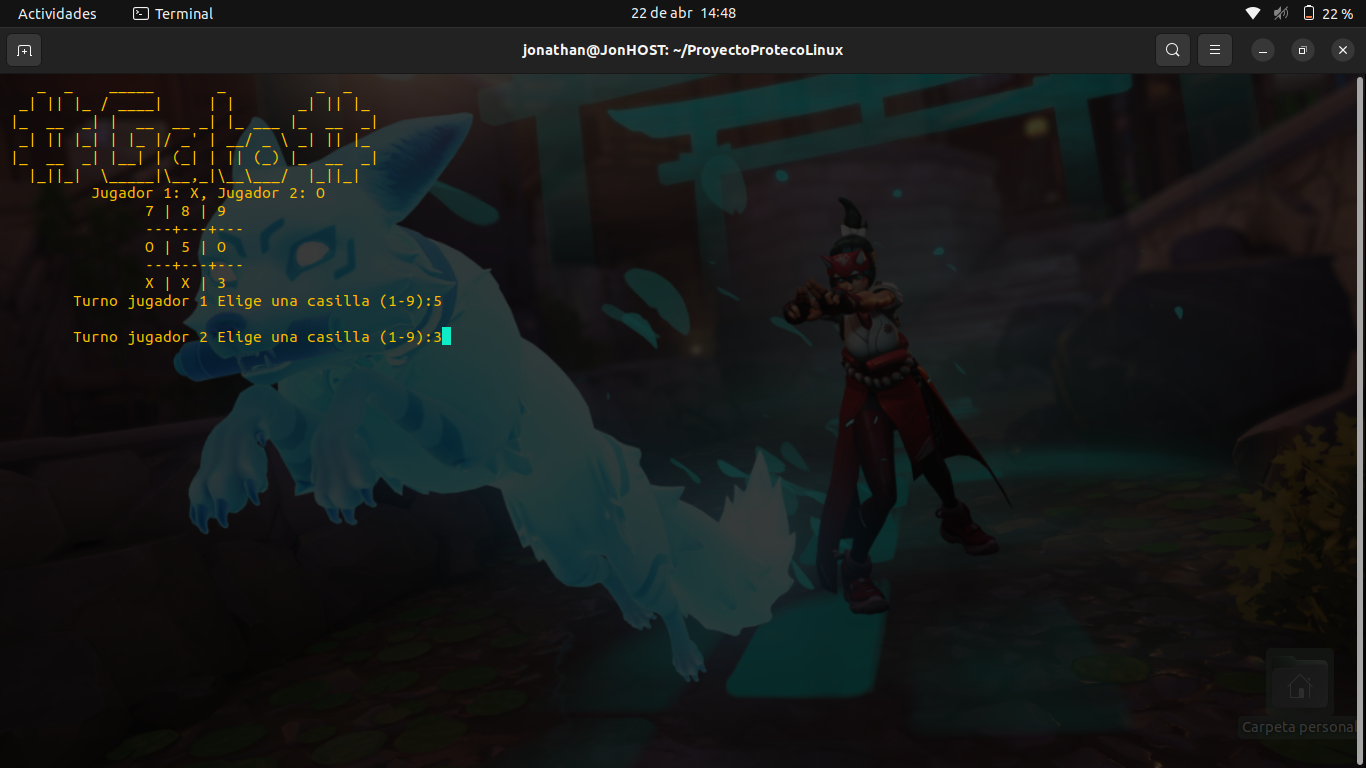
\includegraphics[width=0.5\textwidth]{figurasShell/Jugar5.png}
    \end{figure}
\begin{minted}{bash}
    jugador() {
	local SIMBOLO=$1
	[[ $SIMBOLO == $SIMBOLO_JUGADOR1 ]] && printf "Jugador 1" || printf "Jugador 2"
    }
\end{minted}
    Función para mostrar al ganador
\begin{minted}{bash}
    gana() {
	local GANADOR=$1
	echo "%%%%%%%%%%%%%%%%%%%%%%%%%%%%%%%%%"
	echo "       $(jugador $GANADOR) gana!"
	echo "%%%%%%%%%%%%%%%%%%%%%%%%%%%%%%%%%"
	dibujarTablero
	exit 0
    }
\end{minted}
Función para evaluar casos de victoria

\begin{figure}[H]
    \centering
    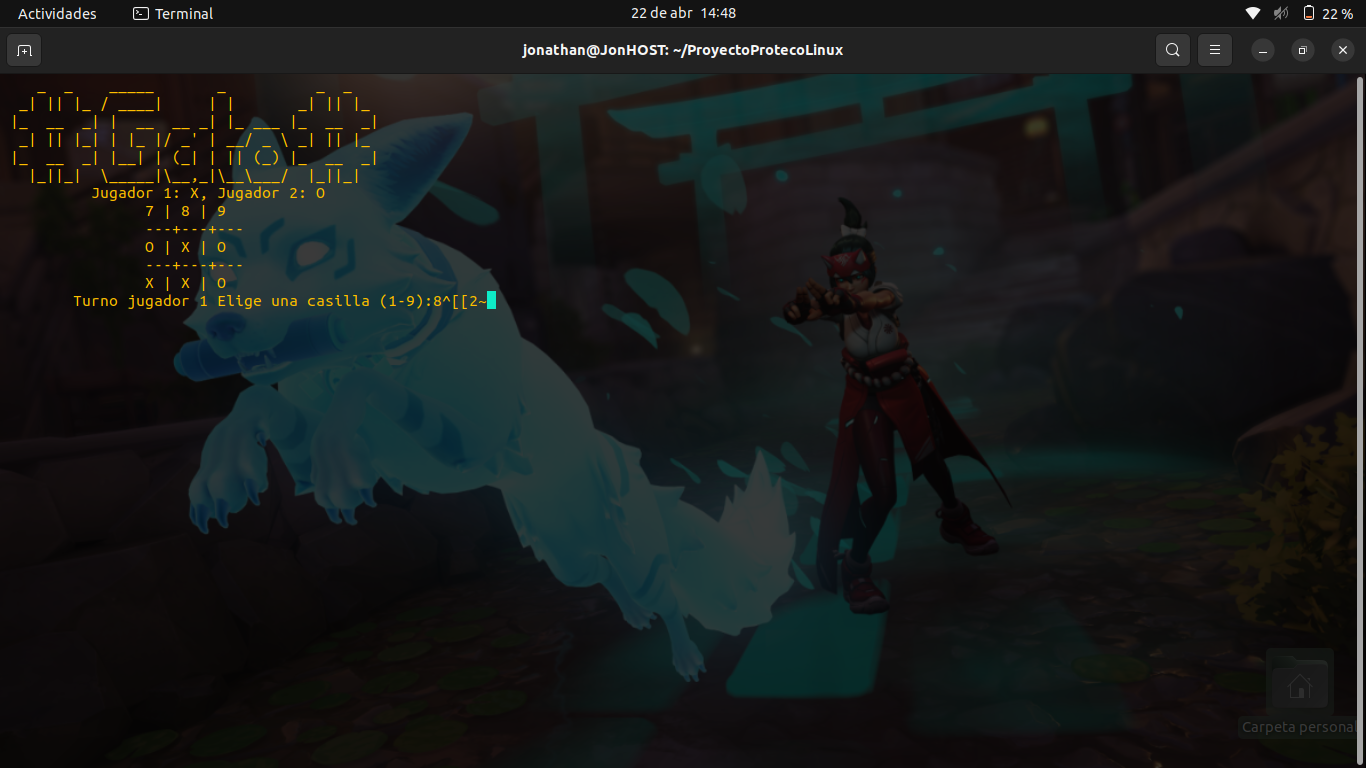
\includegraphics[width=0.5\textwidth]{figurasShell/Jugar6.png}
\end{figure}
\begin{minted}{bash}
    verificarGanador(){
\end{minted}
        Evaluar filas
\begin{minted}{bash}
for i in 1 4 7; do
  j=$(($i + 1))
  k=$(($i + 2))
  GANADOR=${s[$i]}
  [[ ${s[$i]} == ${s[$j]} ]] && [[ ${s[$j]} == ${s[$k]} ]] && gana $GANADOR
done
\end{minted}
	Evaluar columnas
\begin{minted}{bash}
    for i in 1 2 3; do
      j=$(($i + 3))
      k=$(($i + 6))
      GANADOR=${s[$i]}
      [[ ${s[$i]} == ${s[$j]} ]] && [[ ${s[$j]} == ${s[$k]} ]] && gana $GANADOR
done
\end{minted}

Evaluar diagonales

 \begin{minted}{bash}
GANADOR=${s[5]}
[[ ${s[1]} == ${s[5]} ]] && [[ ${s[5]} == ${s[9]} ]]      && gana $GANADOR
[[ ${s[7]} == ${s[5]} ]] && [[ ${s[5]} == ${s[3]} ]]      && gana $GANADOR
}
while true; do
    dibujarTablero
    echo "Turno jugador 1"
    Turno_jugador1
    verificarGanador
    echo ""
    echo "Turno jugador 2"
    Turno_jugador2
    verificarGanador
done

\end{minted}

\begin{figure}[H]
    \centering
    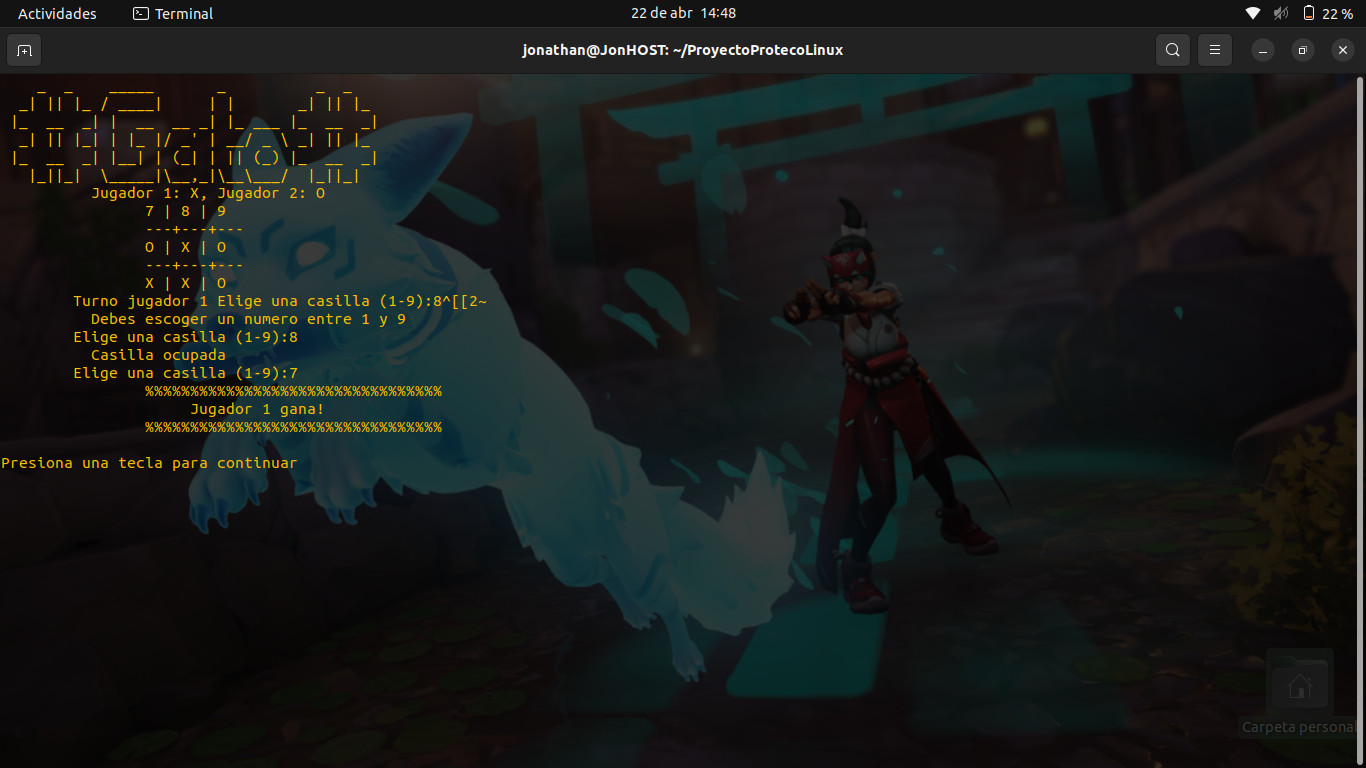
\includegraphics[width=0.5\textwidth]{figurasShell/Jugar7.png}
\end{figure}

\subsection{verificarUsuario.sh}

verificarUsuario.sh es un programa que verifica la identidad del usuario y compara las credenciales que el usuario suministra contra las existentes en el sistema. En esta sección se explica paso a paso la forma en que se logró dicha comparación.

Lo primero que el script hace es solicitar las credenciales del usuario (usuario y contraseña). Estas credenciales deben existir en el sistema.

 \begin{minted}{bash}
    printf "$G Usuario: $W"
    read  usuario
    printf "$G Password: $W"
    read -s password
\end{minted}
\begin{figure}[H]
    \centering
    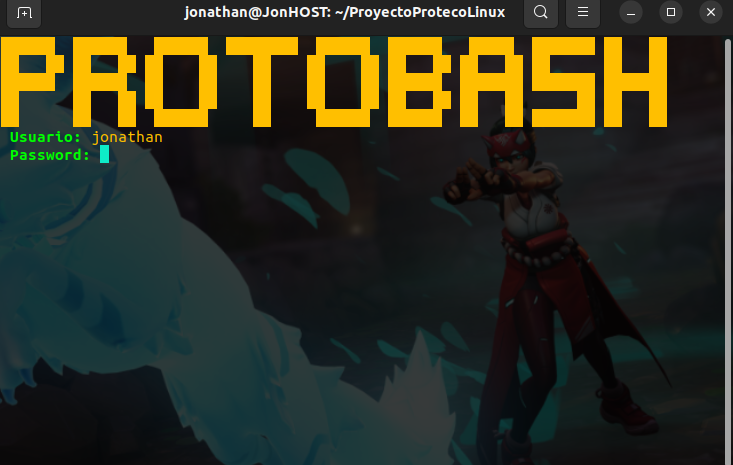
\includegraphics[width=0.5\textwidth]{figurasShell/ProtoBash1.png}
\end{figure}
Aquí es donde empieza lo jugoso del código. Primero, se tiene que acceder al archivo shadow, ubicado en el directorio etc/. De ese archivo se recupera la cantidad de veces que el nombre de usuario aparece para saber si el usuario provisto es correcto.

\begin{minted}{bash}
cadena=`sudo -S grep -r $usuario /etc/shadow`

if [ ${cadena} > 1 ]; then

\end{minted}

Posteriormente, la cadena obtenida con las credenciales del usuario se separan en sub-cadenas, cuyo indicador de separación es el caracter '\$'.  Esta segmentación de la cadena se hace debido a que cada componente tiene información valiosa para poder validar la contraseña provista por el usuario. El primer índice del array contiene el tipo de encriptación utilizada (yescrypt por defecto para Ubunto desde la versión 11). El segundo y tercer índice contienen la \textit{sal} (clave) utilizada para perturbar el algoritmo de encriptación.

\begin{minted}{bash}
IFS='$' read -e -r -a array <<< "$cadena"
salt_hashed="\\$${array[1]}\\$${array[2]}\\$${array[3]}$"    
\end{minted}

Con lo anterior, el siguiente paso es invocar python3 para poder hacer uso del módulo crypt y poder encriptar la contraseña provista por el usuario utilizando el mismo algoritmo y la misma sal para comparar el hash generado.

\begin{minted}{bash}
hash=`python3 -c 'import crypt;import sys;print(crypt.crypt(sys.argv[1],sys.argv[2]));'
$password $salt_hashed`
\end{minted}

Finalmente, con el hash generado y el hash registrado en el sistema, se procede a hacer una comparación de cadenas para determinar si son compatibles.

\begin{minted}{bash}
match=`echo "$cadena" | grep -c "$hash"`
if [ "$match" -eq 1 ]; then
\end{minted}

De esa forma se concluye la forma de hacer la búsqueda del usuario con su contraseña, a partir de sentencias if, con su búsqueda respectiva carácter por carácter para confirmar dicha información.

% enlaces que me van a sirvieron para implementar y documentar esta parte 
% documentación de módulos crypt y sys para python
% crypt https://docs.python.org/es/3/library/crypt.html
% sys https://docs.python.org/3/library/sys.html
% understanding etc/shadow file format on linux https://www.cyberciti.biz/faq/understanding-etcshadow-file/
% Verifying a hashed salted password that uses yescrypt algorithm https://unix.stackexchange.com/questions/707720/verifying-a-hashed-salted-password-that-uses-yescrypt-algorithm
% repo de John y Abraham 

\subsection{sistemaAudio.sh}

En esta parte del sistema se desarrollo un shell script capaz de reproducir por medio de instrucciones básicas en la terminal, intentando realizar lo más cercano a una GUI que se pudo desde una terminal.

Para comenzar la descripción, se incluyeron variables que se usan para identificar los colores que se van a ocupar

\begin{minted}{bash}
# Colores
R='\033[1;31m'
G='\033[1;32m'
B='\033[1;34m'
W='\033[0m'
\end{minted}
\begin{figure}[H]
    \centering
    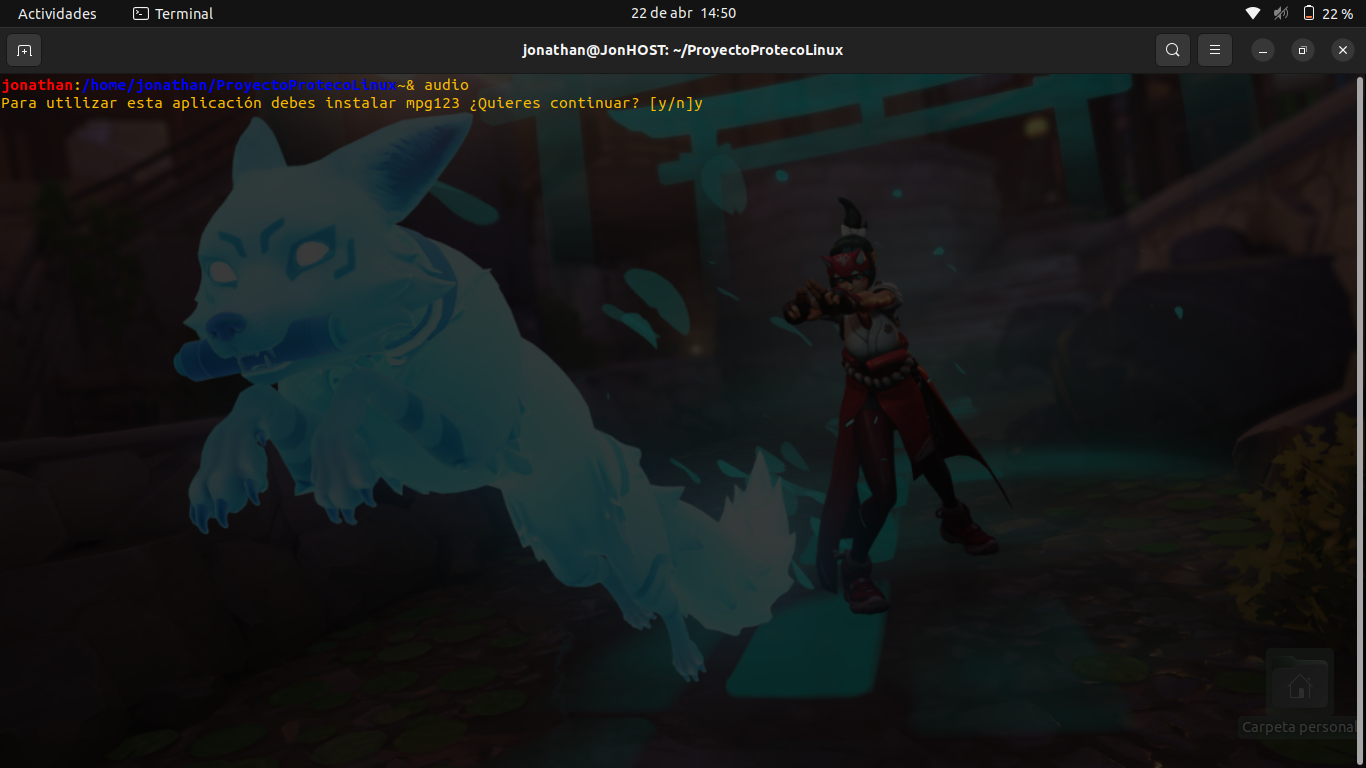
\includegraphics[width=0.5\textwidth]{figurasShell/Audio1.png}
\end{figure}
Continuando podemos observar la dirección del reproductor, en su directorio para guardarlo en una variable y poder ocuparlo después

\begin{minted}{bash}
# Direccion del reproductor
reproductor=/bin/mpg123
\end{minted}

Se verifica que este instalado el reproductor en el directorio, y si no, se prevé esta situación con una instalación posterior para lograr usar el reproductor.
\begin{figure}[H]
    \centering
    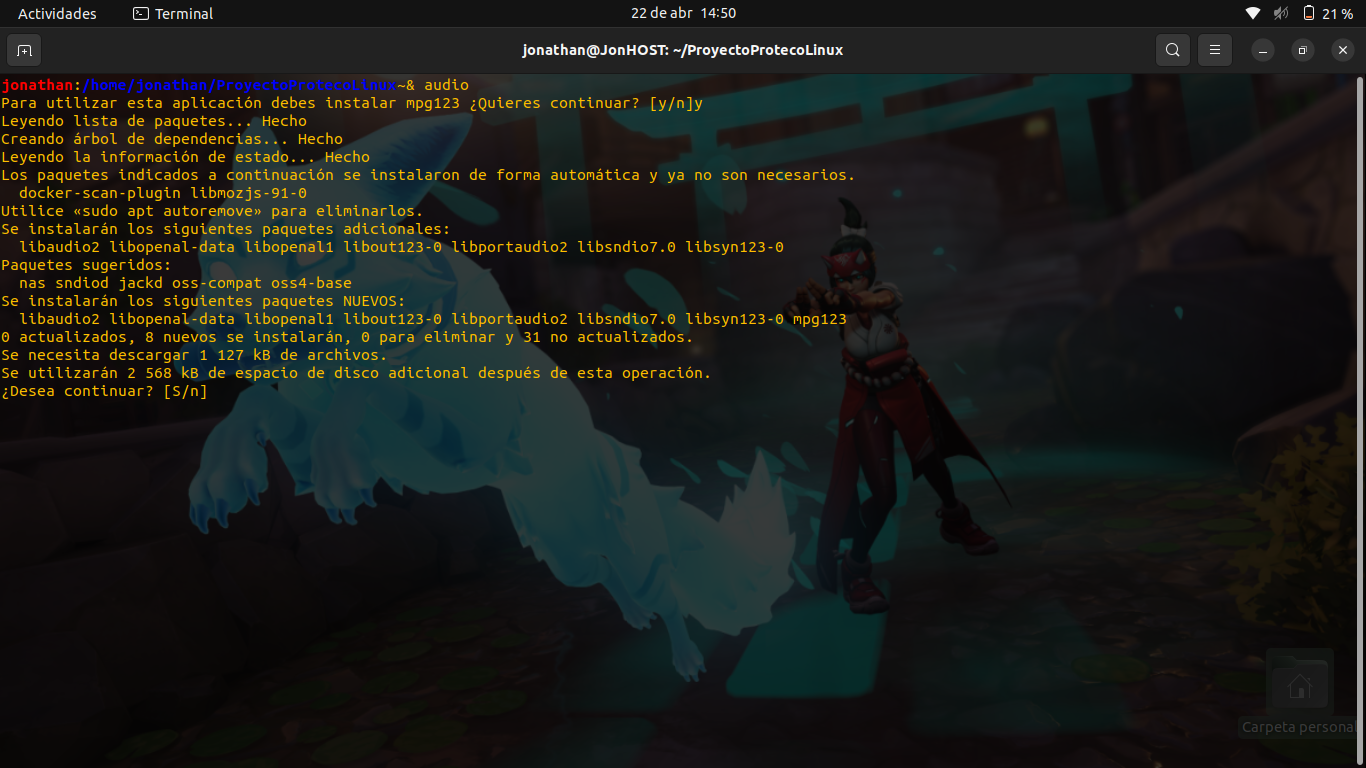
\includegraphics[width=0.5\textwidth]{figurasShell/Audio2.png}
\end{figure}
\begin{minted}{bash}
#Comprobar que si este instalado
if [ ! -f "$reproductor" ];
then
	printf "Para utilizar esta aplicación debes instalar mpg123 ¿Quieres continuar? [y/n]"
       	read instalarYN
   	case $instalarYN in
       		'y') sudo apt install mpg123 ;;
       		'n') exit 0 ;;
       		*) printf "Opción no válida, escribe \'y\' o \'n\'" ;;
	esac
fi

\end{minted}

Después de declarar variables se hace el menú con la petición de escribir los comandos necesarios para su funcionamiento, los cuales se guardan temporalmente en una variable para su uso mientras que no se le de la opción salir.
\begin{figure}[H]
    \centering
    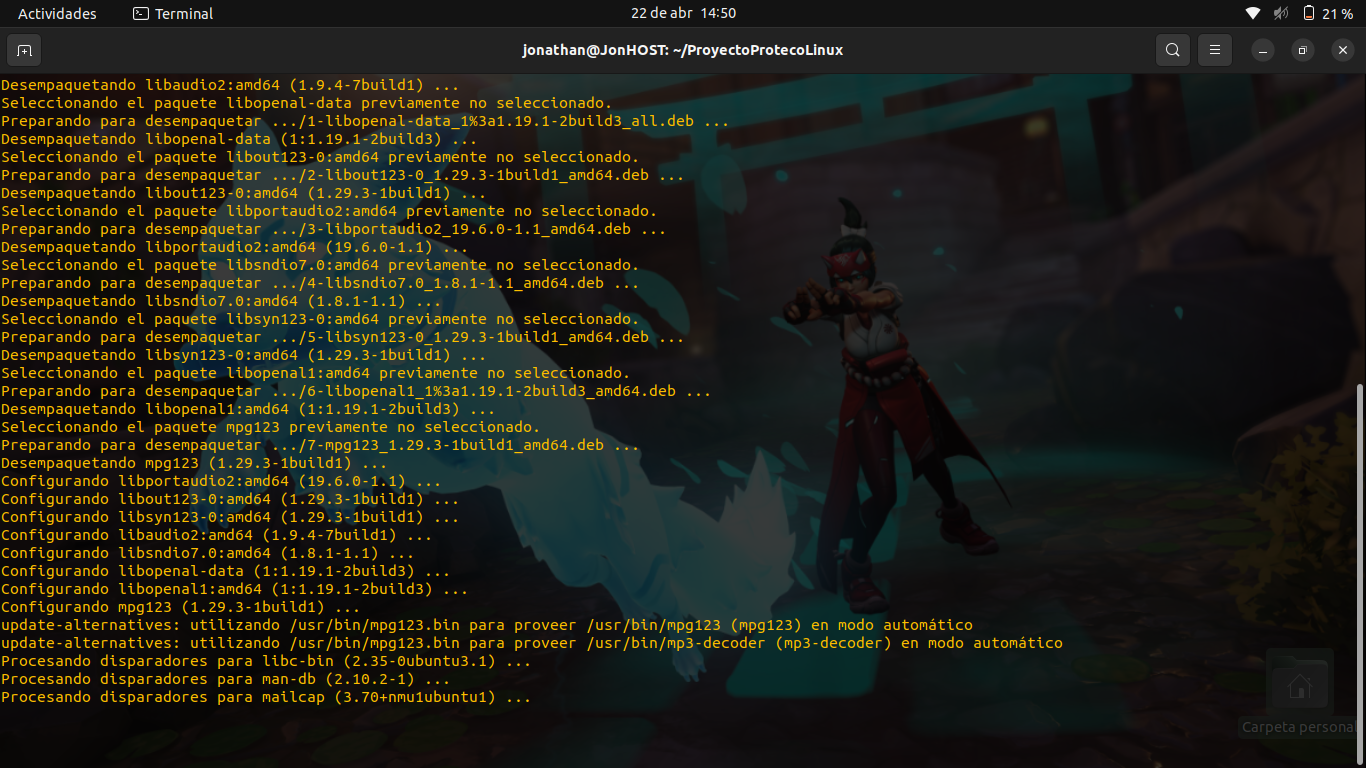
\includegraphics[width=0.5\textwidth]{figurasShell/Audio3.png}
\end{figure}
\begin{minted}{bash}

# Por defecto la musica se toma de la carpeta en el proyecto
dirMusica=musiquitaGratis/


while [ $salir -ne 1 ]
do
	clear
	printf "$R PROTOMIXER\n$W"
	echo "-----------------"
	echo "MENU PRINCIPAL"
	echo "Carpeta actual: $dirMusica"
	echo "1) Reproducir canciones en modo aleatorio"
	echo "2) Cambiar carpeta"
	echo "3) Salir"

	printf "Por favor seleccione una opción\n"
	read -e opcion

	case $opcion in
		1) 
			clear
			echo "		MENU DE REPRODUCCION"
			echo "------------------------------------------"
			echo "		s) Pausar/Reproducir"
			echo "		f) Siguiente"
			echo "		b) Comenzar de nuevo"
			echo "		d) Regresar"
			echo "		q) Detener Reproducción"
			echo "------------------------------------------"
			echo "		CONTROLES ADICIONALES"
			echo "------------------------------------------"
			echo "		+) Subir volumen"
			echo "		-) Bajar volumen"
			echo "		u) Silenciar"
			echo "		l) Listar canciones"
			mpg123 -C --title -q -z "${dirMusica}"/*
			;;
		2) 
			clear
			echo "		  SELECCION DE CARPETA"
			echo "---------------------------------------------------"
			echo "	Ingrese la ruta absoluta o relativa de	"
			echo " 	 de la carpeta donde se encuentre la"
			echo "			música"
			read -e -p "Ruta: " dirMusica
			while [ ! -d $dirMusica ]
			do
				echo "Esa dirección no es válida, inténtalo nuevamente"
				read -e -p "Ruta: " dirMusica
			done
			;;
		3) exit 0 ;;
		*) 
			echo "Opción inválida, elige una opción del menú"
			sleep 1.5
			;;
	esac

done

\end{minted}
\begin{figure}[H]
    \centering
    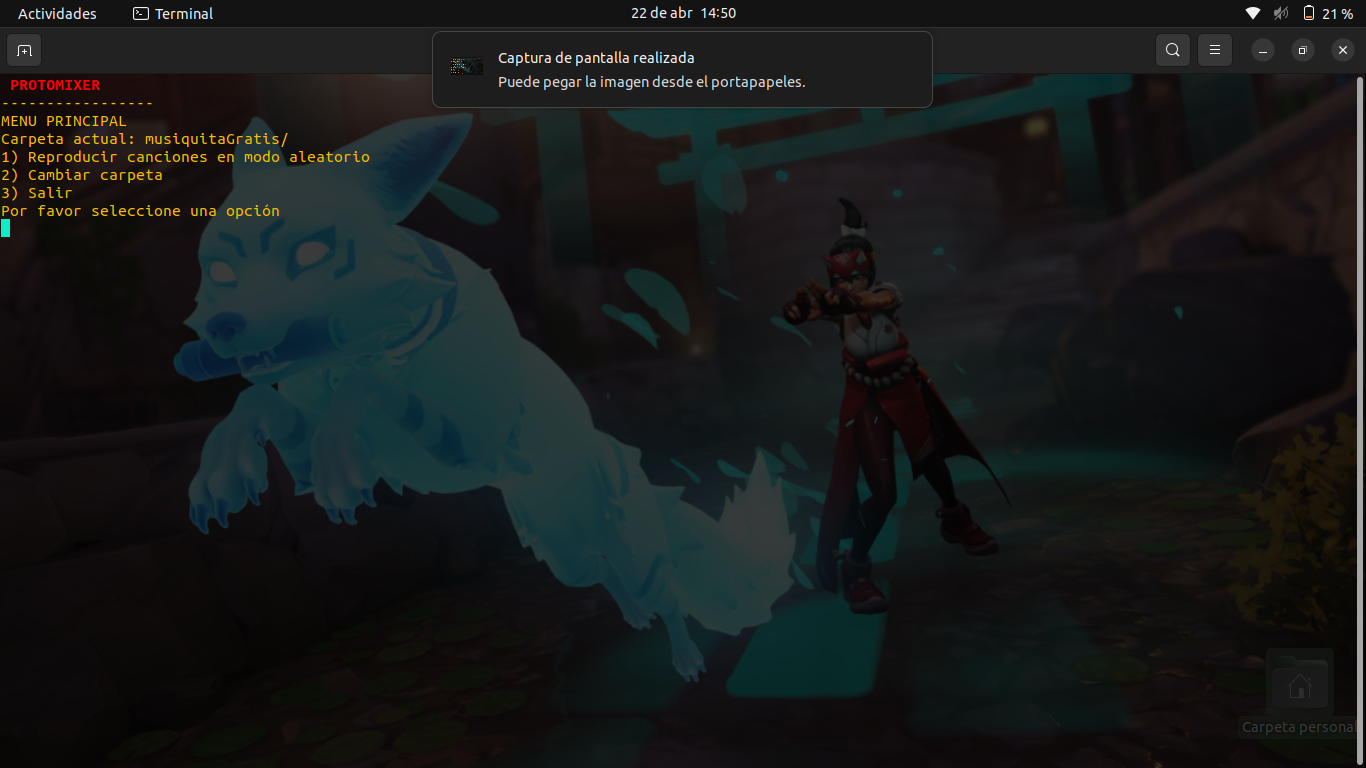
\includegraphics[width=0.5\textwidth]{figurasShell/Audio4.png}
\end{figure}

\begin{figure}[H]
    \centering
    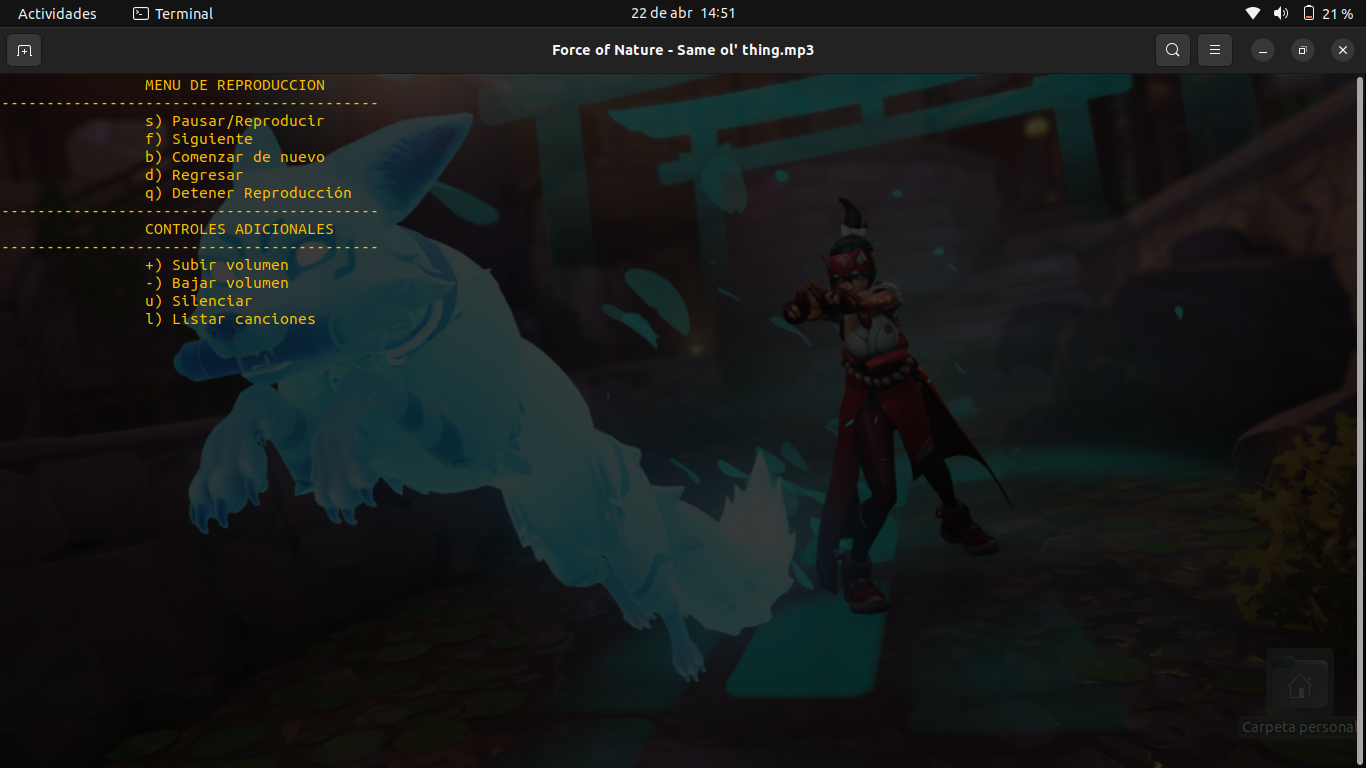
\includegraphics[width=0.5\textwidth]{figurasShell/Audio5.png}
\end{figure}

\begin{figure}[H]
    \centering
    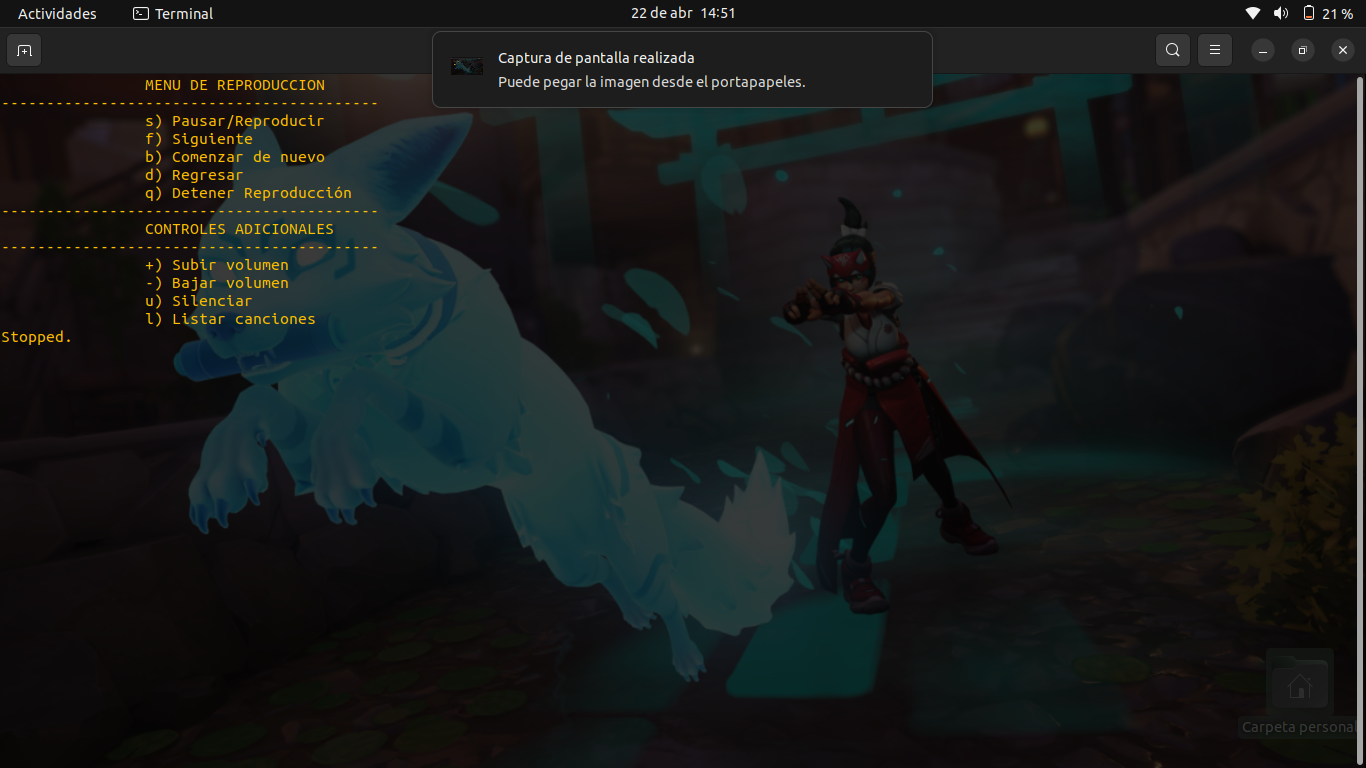
\includegraphics[width=0.5\textwidth]{figurasShell/Audio6.png}
\end{figure}

\begin{figure}[H]
    \centering
    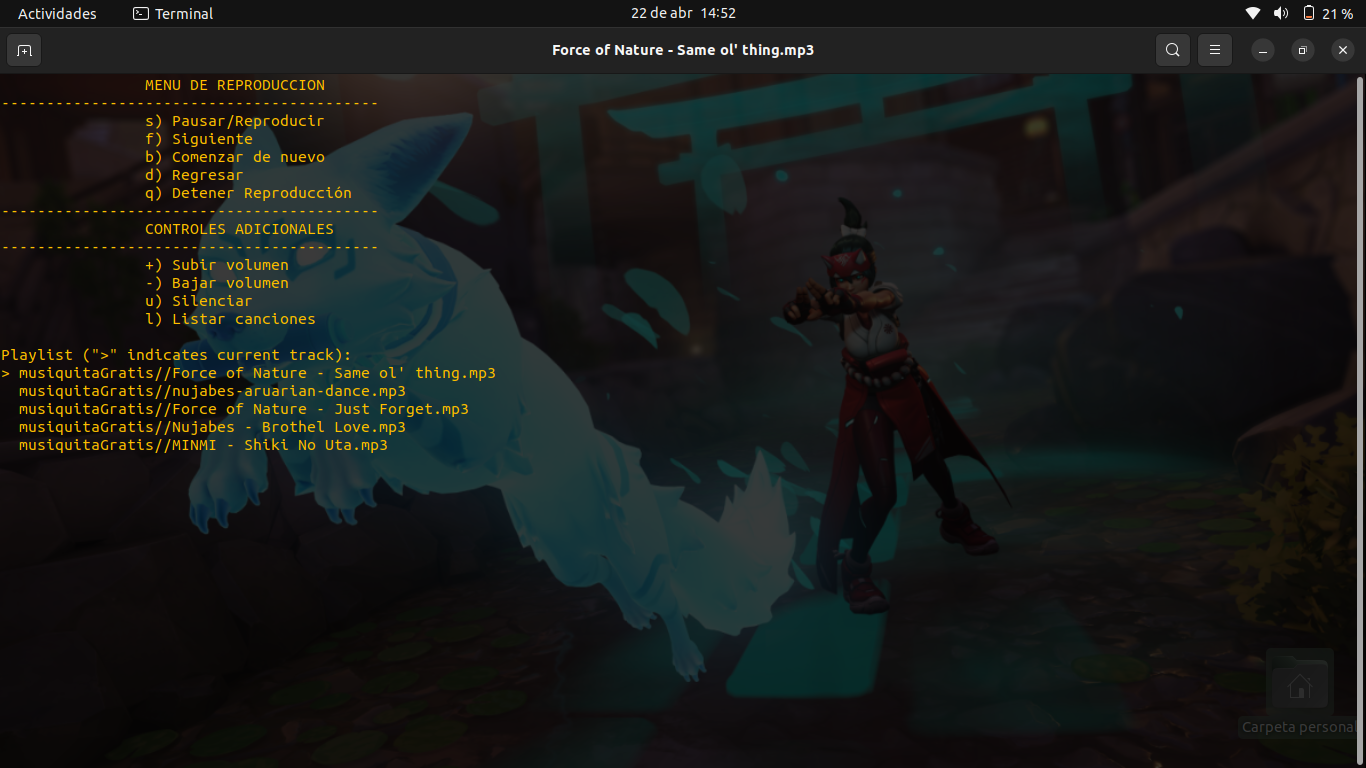
\includegraphics[width=0.5\textwidth]{figurasShell/Audio7.png}
\end{figure}

\begin{figure}[H]
    \centering
    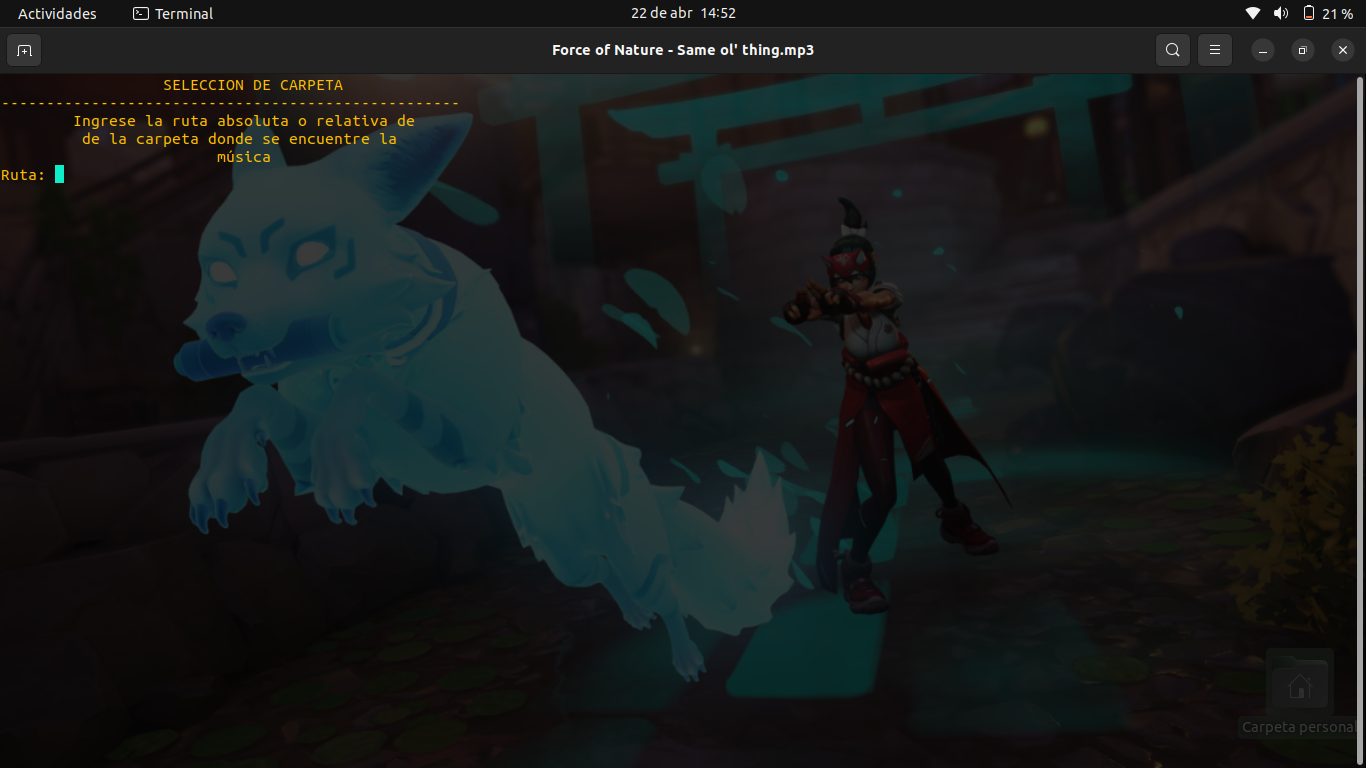
\includegraphics[width=0.5\textwidth]{figurasShell/Audio8.png}
\end{figure}

\begin{figure}[H]
    \centering
    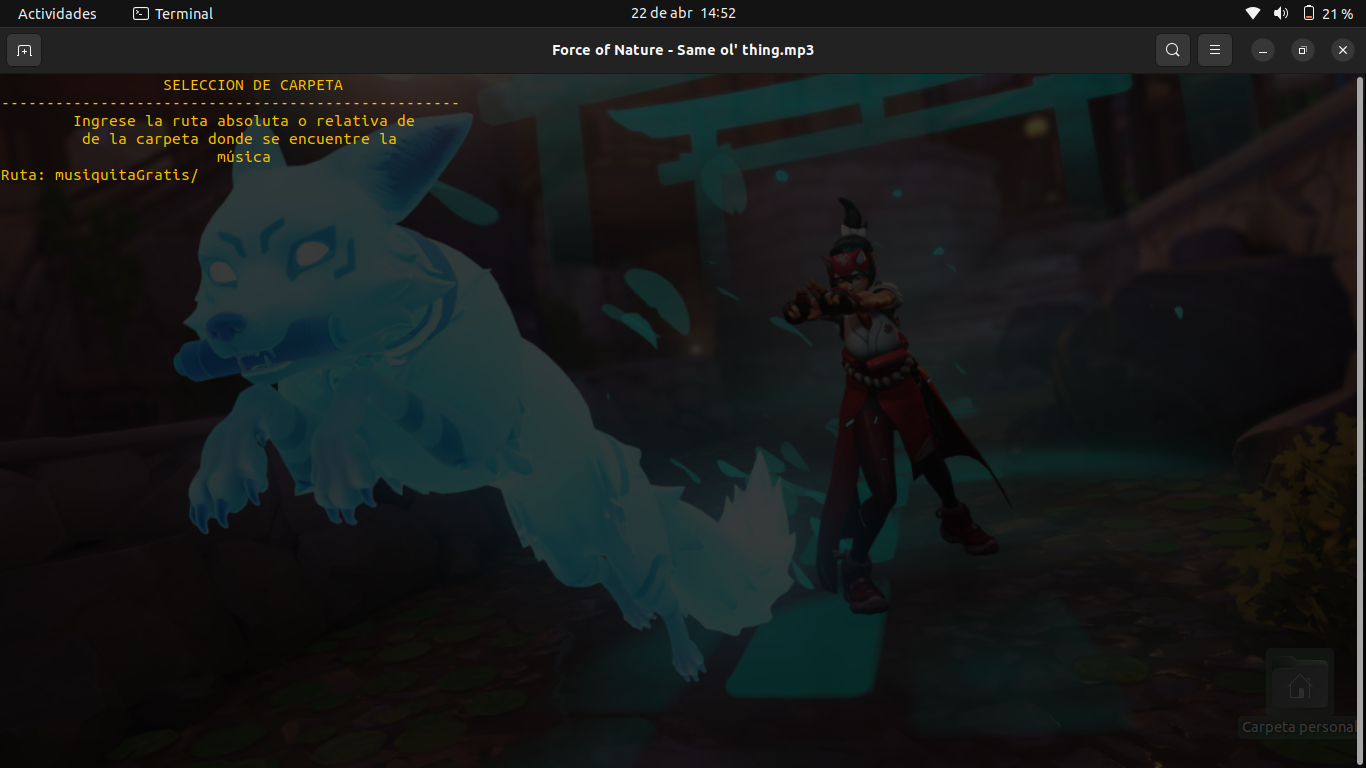
\includegraphics[width=0.5\textwidth]{figurasShell/Audios9.png}
\end{figure}

\begin{figure}[H]
    \centering
    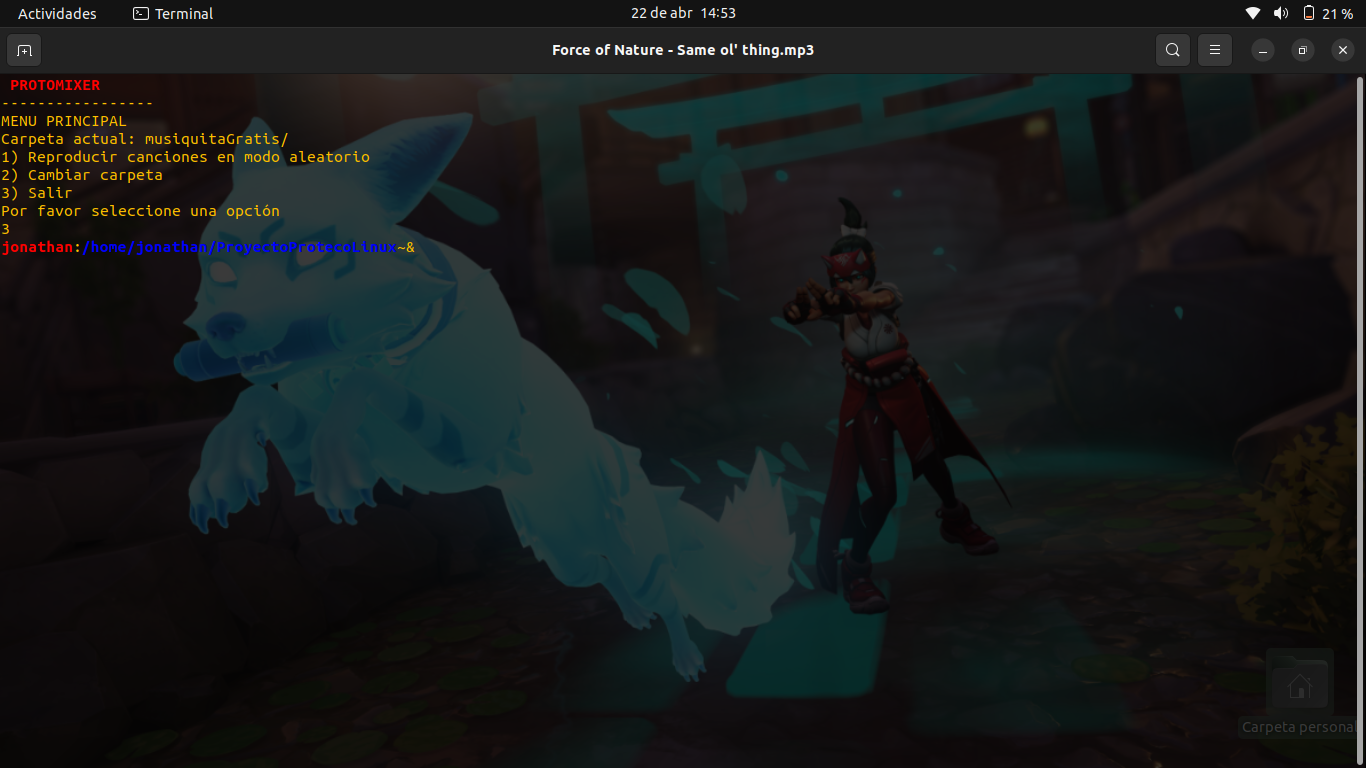
\includegraphics[width=0.5\textwidth]{figurasShell/Audio10.png}
\end{figure}
\section{Conclusión}

\subsection{Alan Carrasco}

En este proyecto se realizó una terminal de comandos capaz de interpretar comandos personalizados y los propios del sistema operativo. Las funciones personalizadas que se pueden ejecutar con esta terminal son, como ya se mencionó, buscar, infosis, ayuda, créditos, tiempo, jugar y audio. Cabe mencionar que el proyecto tiene sus limitaciones tanto funcionales, como estéticas. Sin embargo, para haber tomado un curso muy intensivo sobre GNU/Linux y jamás haber hecho cosas como encriptación o uso de programas para audio desde terminal, resultó muy enriquecedor.

Finalmente, quiero agradecer a los instructores de Linux por haber hecho su mejor esfuerzo por transmitirnos sus conocimientos; a mi buddy y a mis demás compañeros por haber colaborado y llegar a soluciones juntos; y a todas las personas que comparten sus proyectos y conocimientos en internet. Sin alguno de ellos este proyecto no se habría podido llevar a cabo. Gracias.

\subsection{Jonathan García}

Puedo decir que el proyecto fue bastante laborioso y en parte difícil por la búsqueda de información, de incorporar esta información y claro, contemplar cada uno de los archivos para su acoplamiento correcto y uso correcto de cada una de estas funciones en los diferentes archivos que teníamos, tanto de tipo shell script como de tipo txt.

Contemplar en su mayoria, todos los requerimentos establecidos en el proyecto como lograr esa cohesión entre lo trabajado con mi buddy y lo que yo hice, fue algo bastante satisfactorio por el hecho de ver los resultados y lograr hacer un proyecto de calidad y diseño único. 


\end{document}
